\section{\Large PROBLEM SET 3}
\subsection{Problem 3}

\subsubsection{Impose that satellite is axial-symmetric (i.e., impose $I_x=I_y\neq I_z$). Repeat numerical simulation from previous pset using initial condition 4) from previous pset.}

The principal inertia of the Aqua satellite is listed in \ref{sec:principal_inertia_def_and_calc}. Imposing that $I_y=I_x$, the axis-symmetric representation of the satellite is seen below.

\begin{equation*}
    \boldsymbol{I_{CM}'} = \begin{bmatrix}
        17510 & 0 & 0 \\
        0 & 17510 & 0 \\
        0 & 0 & 36245
    \end{bmatrix} \text{kg} \cdot \text{m}^2
\end{equation*}

The torque-free simulation results can be seen in Figure \ref{fig:axis_symmetric_magnitudes}.

\subsubsection{Program analytical solution for axial-symmetric satellite. Compute it at same time steps and from same initial conditions.}

The analytical solution for an axis symmetric satellite in torque-free motion comes from Equations \ref{eq:axis_symmetric_1} -- \ref{eq:axis_symmetric_3}.
\begin{eqnarray}
    I_x \dot{\omega}_x + (I_z - I_x) \omega_y \omega_z &= 0 \label{eq:axis_symmetric_1}\\
    I_y \dot{\omega}_y + (I_x - I_z) \omega_z \omega_x &= 0 \label{eq:axis_symmetric_2}\\
    I_z \dot{\omega}_z &= 0 \label{eq:axis_symmetric_3}
\end{eqnarray}
An immediately apparent conclusion is that $\omega_z$ remains constant. That is, $\omega_z = \omega_z(t = 0) = \omega_{z,0}$. Let $\lambda = (I_z - I_x) \omega_{z,0}/ I_x$. This results in the following relations.
\begin{eqnarray*}
    \dot{\omega}_x + \lambda \omega_y &= 0 \\
    \dot{\omega}_y - \lambda \omega_x &= 0
\end{eqnarray*}
Two conclusion can be pulled from this. The first is that $\omega_x^2 + \omega_y^2 = \text{const}$. That is, the norm of the 2D vector composed of x and y components of the angular velocity of the spacecraft is constant. Furthermore, the claim can be made that this vector rotations about the z-axis at a rate of $\lambda$ given in radians per second. The evolution of the x and y components of angular velocity over time given initial conditions $\omega_x (t = 0) = \omega_{x,0}$ and $\omega_y (t = 0) = \omega_{y,0}$ are shown below.
\begin{eqnarray*}
    \omega_x(t) &= \omega_{x,0} \cos{\lambda t} - \omega_{y,0} \sin{\lambda t} \\
    \omega_y(t) &= \omega_{x,0} \sin{\lambda t} + \omega_{y,0} \cos{\lambda t}
\end{eqnarray*}
Therefore the overall vector valued solution is seen in Equation \ref{eq:axis_symmetric_result}.

\begin{equation} \label{eq:axis_symmetric_result}
    \vec{\omega}(t) = \begin{bmatrix}
        \omega_{x,0} \cos{\lambda t} - \omega_{y,0} \sin{\lambda t} &
        \omega_{x,0} \sin{\lambda t} + \omega_{y,0} \cos{\lambda t} & \omega_{z,0}
    \end{bmatrix}^T
\end{equation}

The results of this equation evaluated at the same time steps as the simulation can also be seen in \ref{fig:axis_symmetric_magnitudes}

The

\subsubsection{Compare numerical and analytical solutions. Plot differences (errors), do not only superimpose absolute values. Tune numerical integrator for large discrepancies. Are angular velocity vector and angular momentum vector changing according to theory in principal axes?}

The vector components for both the simulated results and analytical results for axis-symmetric torque-free motion of the Aqua satellite are presented in Figure \ref{fig:axis_symmetric_magnitudes}. The component-wise errors plotted over time are also presented below in Figure \ref{fig:axis_symmetric_errors}. 

\begin{figure} [H]
    \centering
    \captionsetup{justification = centering}
    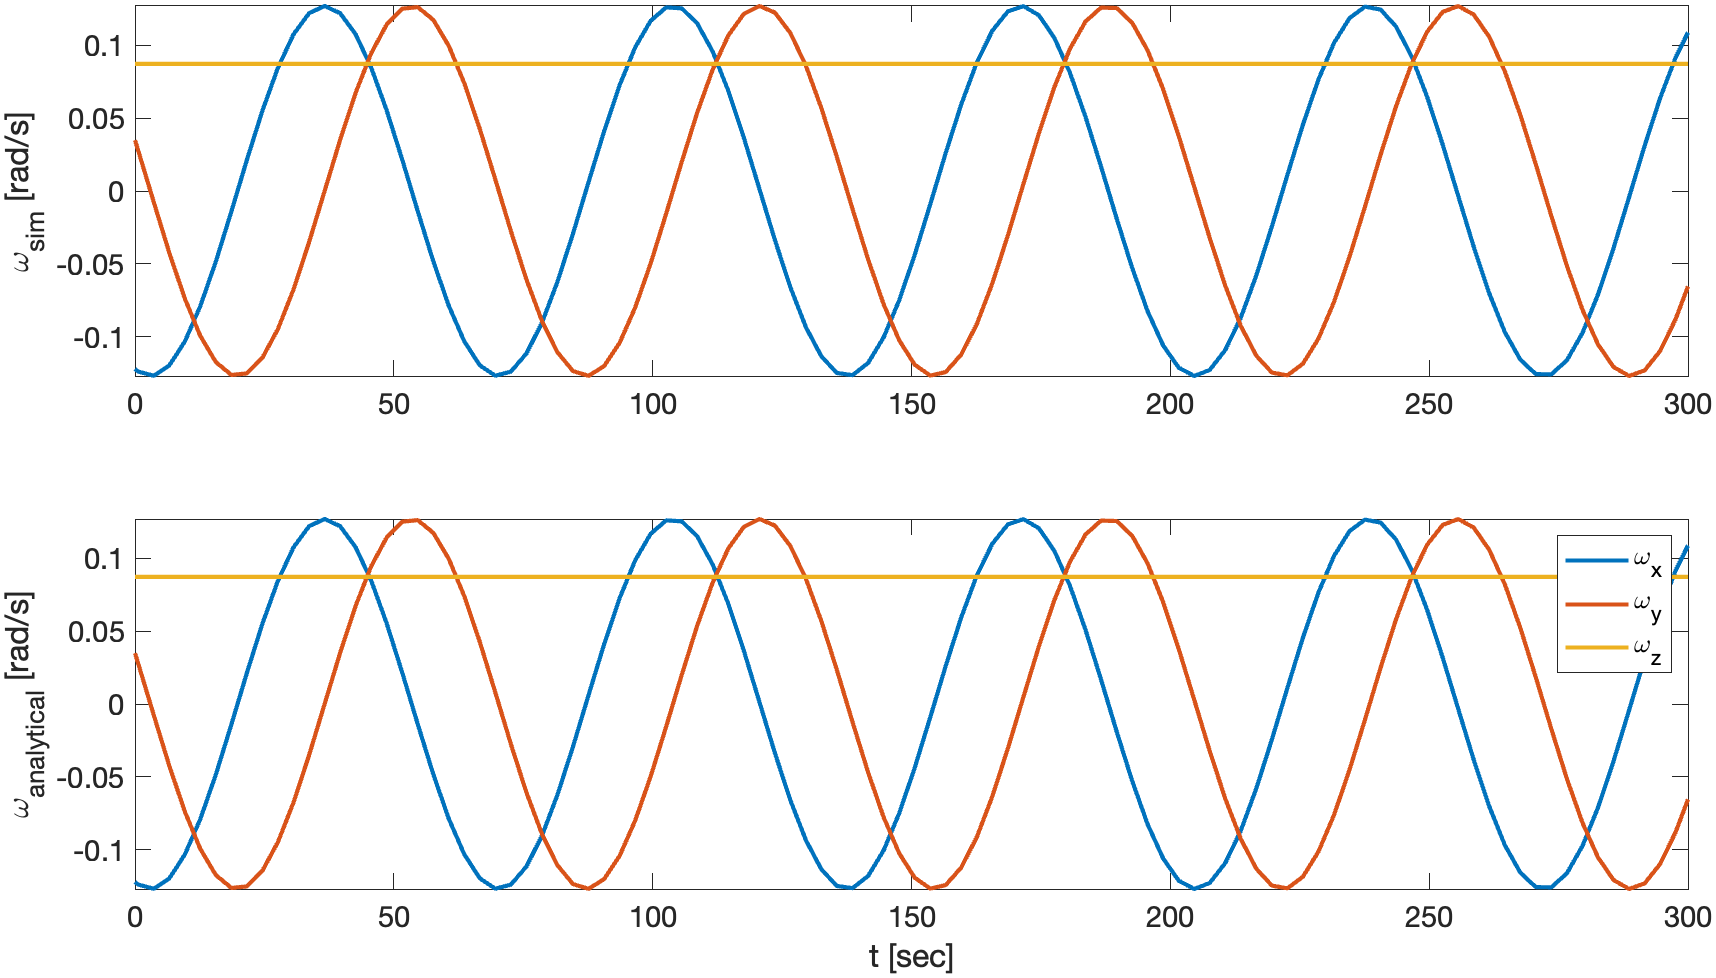
\includegraphics[width = 10cm] {Images/sim_vs_anlt_magnitude.png}
    \caption{Angular Velocity Vector Components for Axis-Symmetric Torque-Free Motion over Time for Simulation (top) and Analytical (bottom) Solutions}
    \label{fig:axis_symmetric_magnitudes}
\end{figure}

\begin{figure} [H]
    \centering
    \captionsetup{justification = centering}
    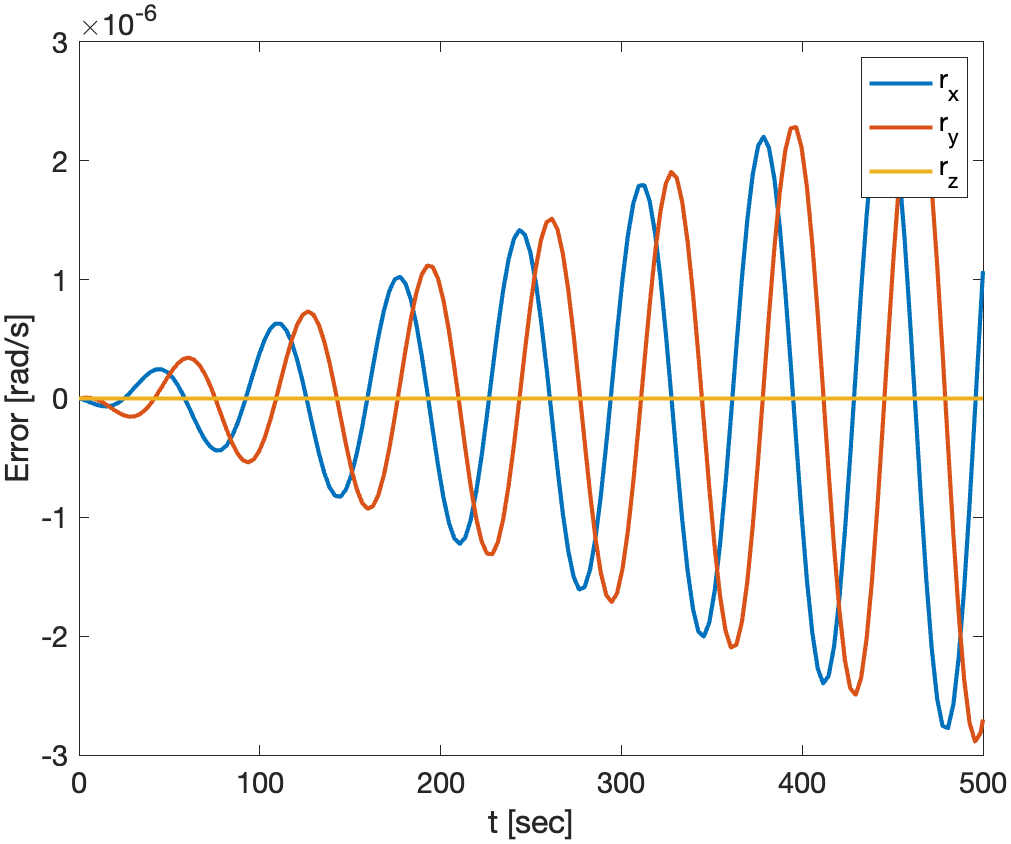
\includegraphics[width = 10cm] {Images/sim_vs_anlt_error.png}
    \caption{Component-wise Velocity Errors for Axis-Symmetric Torque-Free Motion over Time for Simulation vs. Analytical Solutions}
    \label{fig:axis_symmetric_errors}
\end{figure}

The small error in each component suggests that the behavior of the satellite in simulation follows the expected analytical solution. The simulation does tend to diverge from the analytical solution over time at a roughly linear rate. This error growth might be mitigated via further tuning of the step size and tolerances within the numerical integration.

\subsubsection{Program Kinematic equations of motion correspondent to a nominal attitude parameterization of your choice.}

The nominal attitude parametrization for the Aqua satellite is a 313 Euler Angle representation. 

The rotation matrix $\boldsymbol{R}$ that defines the orientation of a body fixed frame on the satellite with respect to an inertial frame behaves as described in Equations \ref{eq:inertial_to_body} and \ref{eq:body_to_inertial} where an arbitrary vector $\vec{v}_I$ is in the inertial frame and $\vec{v}$ is in a body fixed frame of interest. Equation \ref{eq:body_to_inertial} holds the implicit assumption that $\boldsymbol{R}$ is an orthogonal matrix. 
\begin{eqnarray}
    \vec{v} &= \boldsymbol{R} \vec{v}_I \label{eq:inertial_to_body} \\
    \vec{v}_I &= \boldsymbol{R}^T \vec{v} \label{eq:body_to_inertial}
\end{eqnarray}
\subsubsection{Program Kinematic equations of motion correspondent to a different attitude parameterization from the previous step. This is used for comparison, to get familiar with different approaches, and as fall back solution in the case of singularities.}

A secondary paramterization of the spacecraft attitude utilizes quaternions. Quaternions are composed of a scalar component $q_0$ and a vector component $\vec{q} = \begin{bmatrix}  q_1 & q_2 & q_3  \end{bmatrix}^T$. In short $q = \{q_0, \vec{q}\}$. 

To propagate the spacecraft state in terms of this attitude representation, the rate change of all components of the quaternion is represented by Equation \ref{eq:quat_rate_change}. The vector concatentation of the scalar component with the vector component of the quaternion is given by $q_{0:3}$, and the angular velocity is represented in the body fixed frame.

\begin{equation} \label{eq:quat_rate_change}
    \dot{q}_{0:3} = \frac{1}{2} \boldsymbol{W}^T \vec{\omega}
\end{equation}

The matrix $\boldsymbol{W}$ referenced in the above equation is defined as follows.

\begin{equation*}
    \boldsymbol{W} = \begin{bmatrix}
        -q_1 & q_0 & q_3 & -q_2 \\
        -q_2 & -q_3 & q_0 & q_1 \\
        -q_3 & q_2 & -q_1 & q_0
    \end{bmatrix}
\end{equation*}

The rotation matrix $\boldsymbol{R}$ that represents the rotation between the body fixed from and the inertial frame is defined as follows.

\begin{equation*}
    \boldsymbol{R} = \begin{bmatrix}
        q_0^2 + q_1^2 - q_2^2 - q_3^2 & 2(q_1q_2 + q_0q_3) & 2(q_1q_3 - q_0q_2) \\
        2(q_1q_2 - q_0q_3) & q_0^2 - q_1^2 + q_2^2 - q_3^2 & 2(q_2q_3 + q_0q_1) \\
        2(q_1q_3 + q_0q_2) & 2(q_2q_3 - q_0q_1) & q_0^2 - q_1^2 - q_2^2 + q_3^2
    \end{bmatrix}
\end{equation*}

Therefore, knowing the angular velocity of the spacecraft at each point in time, the rate change of the quaternion components can be computed. Therefore, the entire attitude state can be propagated.

\subsubsection{Go back to your original satellite inertia tensor. Numerically integrate Euler AND Kinematic equations from arbitrary initial conditions (warning: stay far from singularity of adopted parameterization). Multiple revolutions. The output is the evolution of the attitude parameters over time. These attitude parameters describe orientation of principal axes relative to inertial axes.}

The time history of Euler angles versus time can be seen plotted in \ref{}.

Additionally, a time history of all quaternion components can be seen plotted against time in Figure \ref{fig:time_history_quaternion}. 

\begin{figure} [H]
    \centering
    \captionsetup{justification = centering}
    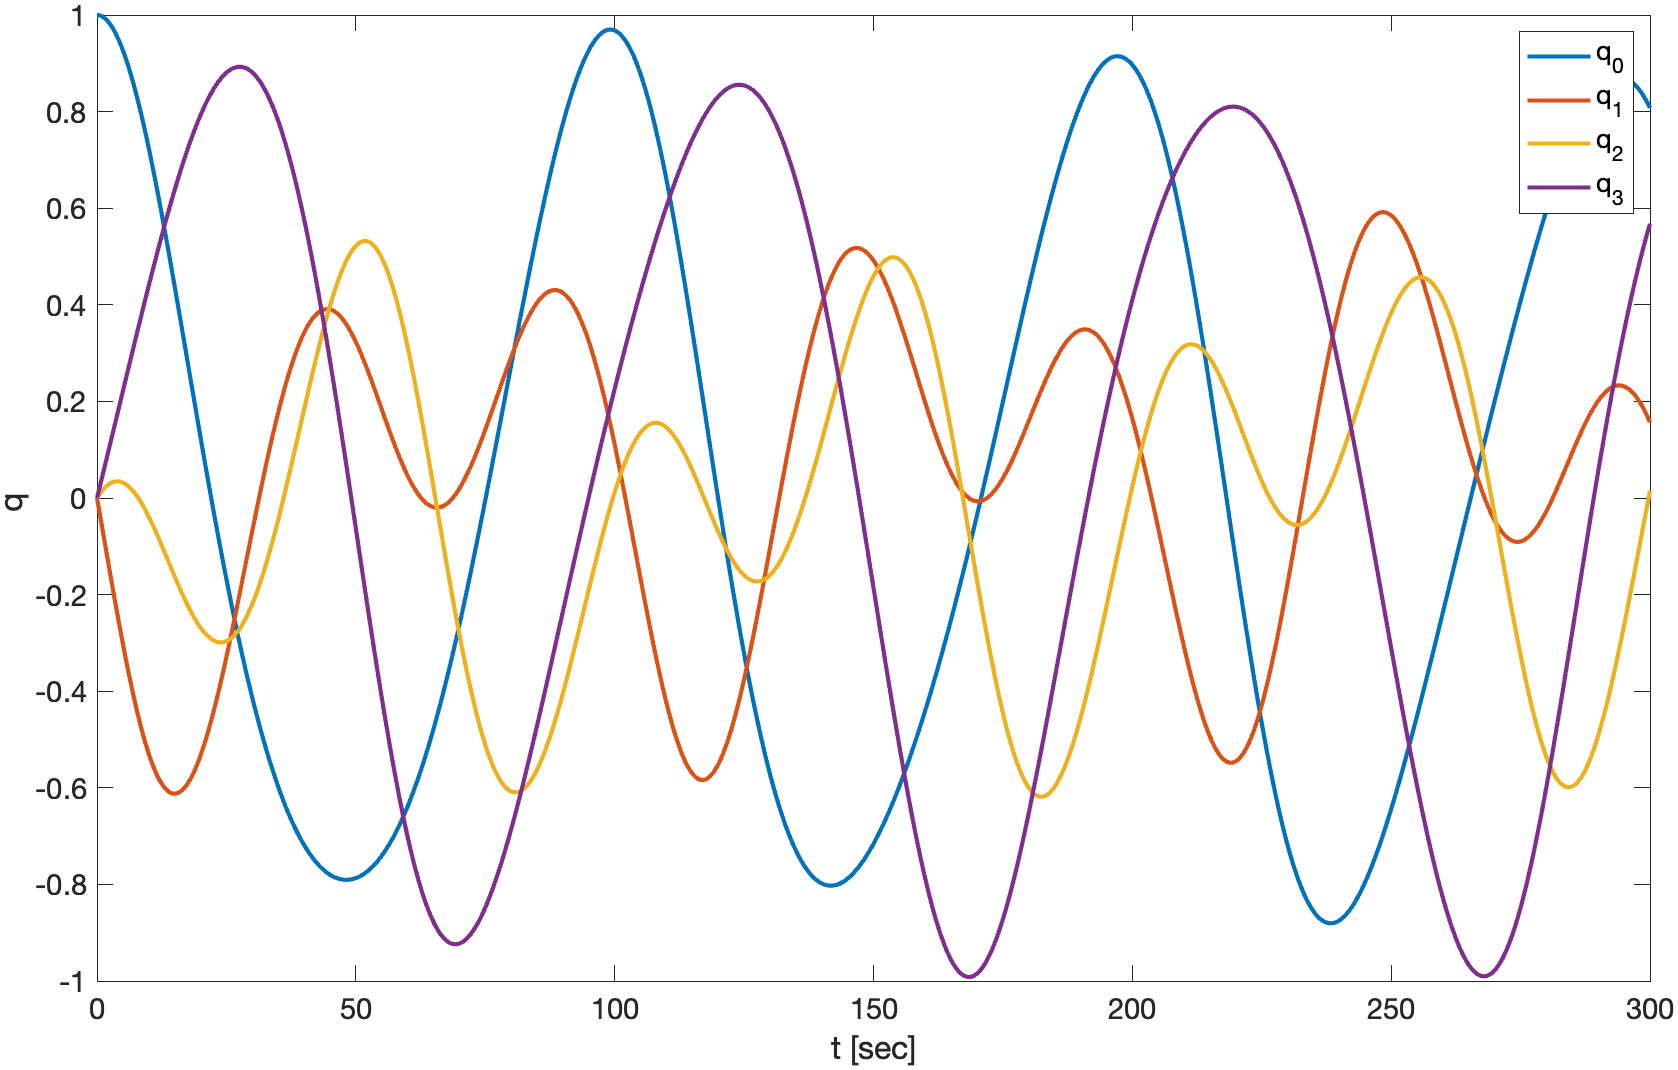
\includegraphics[width = 10cm] {Images/time_history_quat.png}
    \caption{Time History of Quaternion Components}
    \label{fig:time_history_quaternion}
\end{figure}

\subsubsection{Since inertial position, velocity, and attitude, are known at the same time throughout the simulation, it is now possible to express vectors in the reference systems of interest}

To compute the angular momentum in the inertial frame, the angular momentum must first be computed in the principal axis frame. This momentum vector is then rotation using the rotation matrix $\boldsymbol{R}$ using Equation \ref{eq:body_to_inertial}. This is done for each time step in the simulation. and the path traced by the tip of the vector is plotted in Figure \ref{}. 

\paragraph{Compute angular momentum vector in inertial coordinates and verify that it is constant (not only its magnitude as in PS2) by plotting its components.}

\paragraph{Compute angular velocity vector in inertial coordinates and plot the herpolhode in 3D (line drawn in inertial space by angular velocity). Is the herpolhode contained in a plane perpendicular to the angular momentum vector? Show it}

\paragraph{Compute and plots unit vectors of orbital frame, body axes, and principal axes in 3D as a function of time in inertial coordinates. (Be creative on how to show moving vectors in 3D).}